Tunel $ \Tau $ v molekule je v našem případě modelován posloupností koulí o různých poloměrech umístěných v prostoru. Pro posloupnost koulí $ \Tau = \{S_i\}_{i=0}^{n} $ navíc platí $ S_i \bigcap S_{i+1} \neq \emptyset $ pro všechna $ 0 \leq i < n $.
Pro představu jak takový tunel může vypadat uvádíme obrázek \ref{fig:basic_tunnel}.
\begin{figure}[ht]
  	\centering
	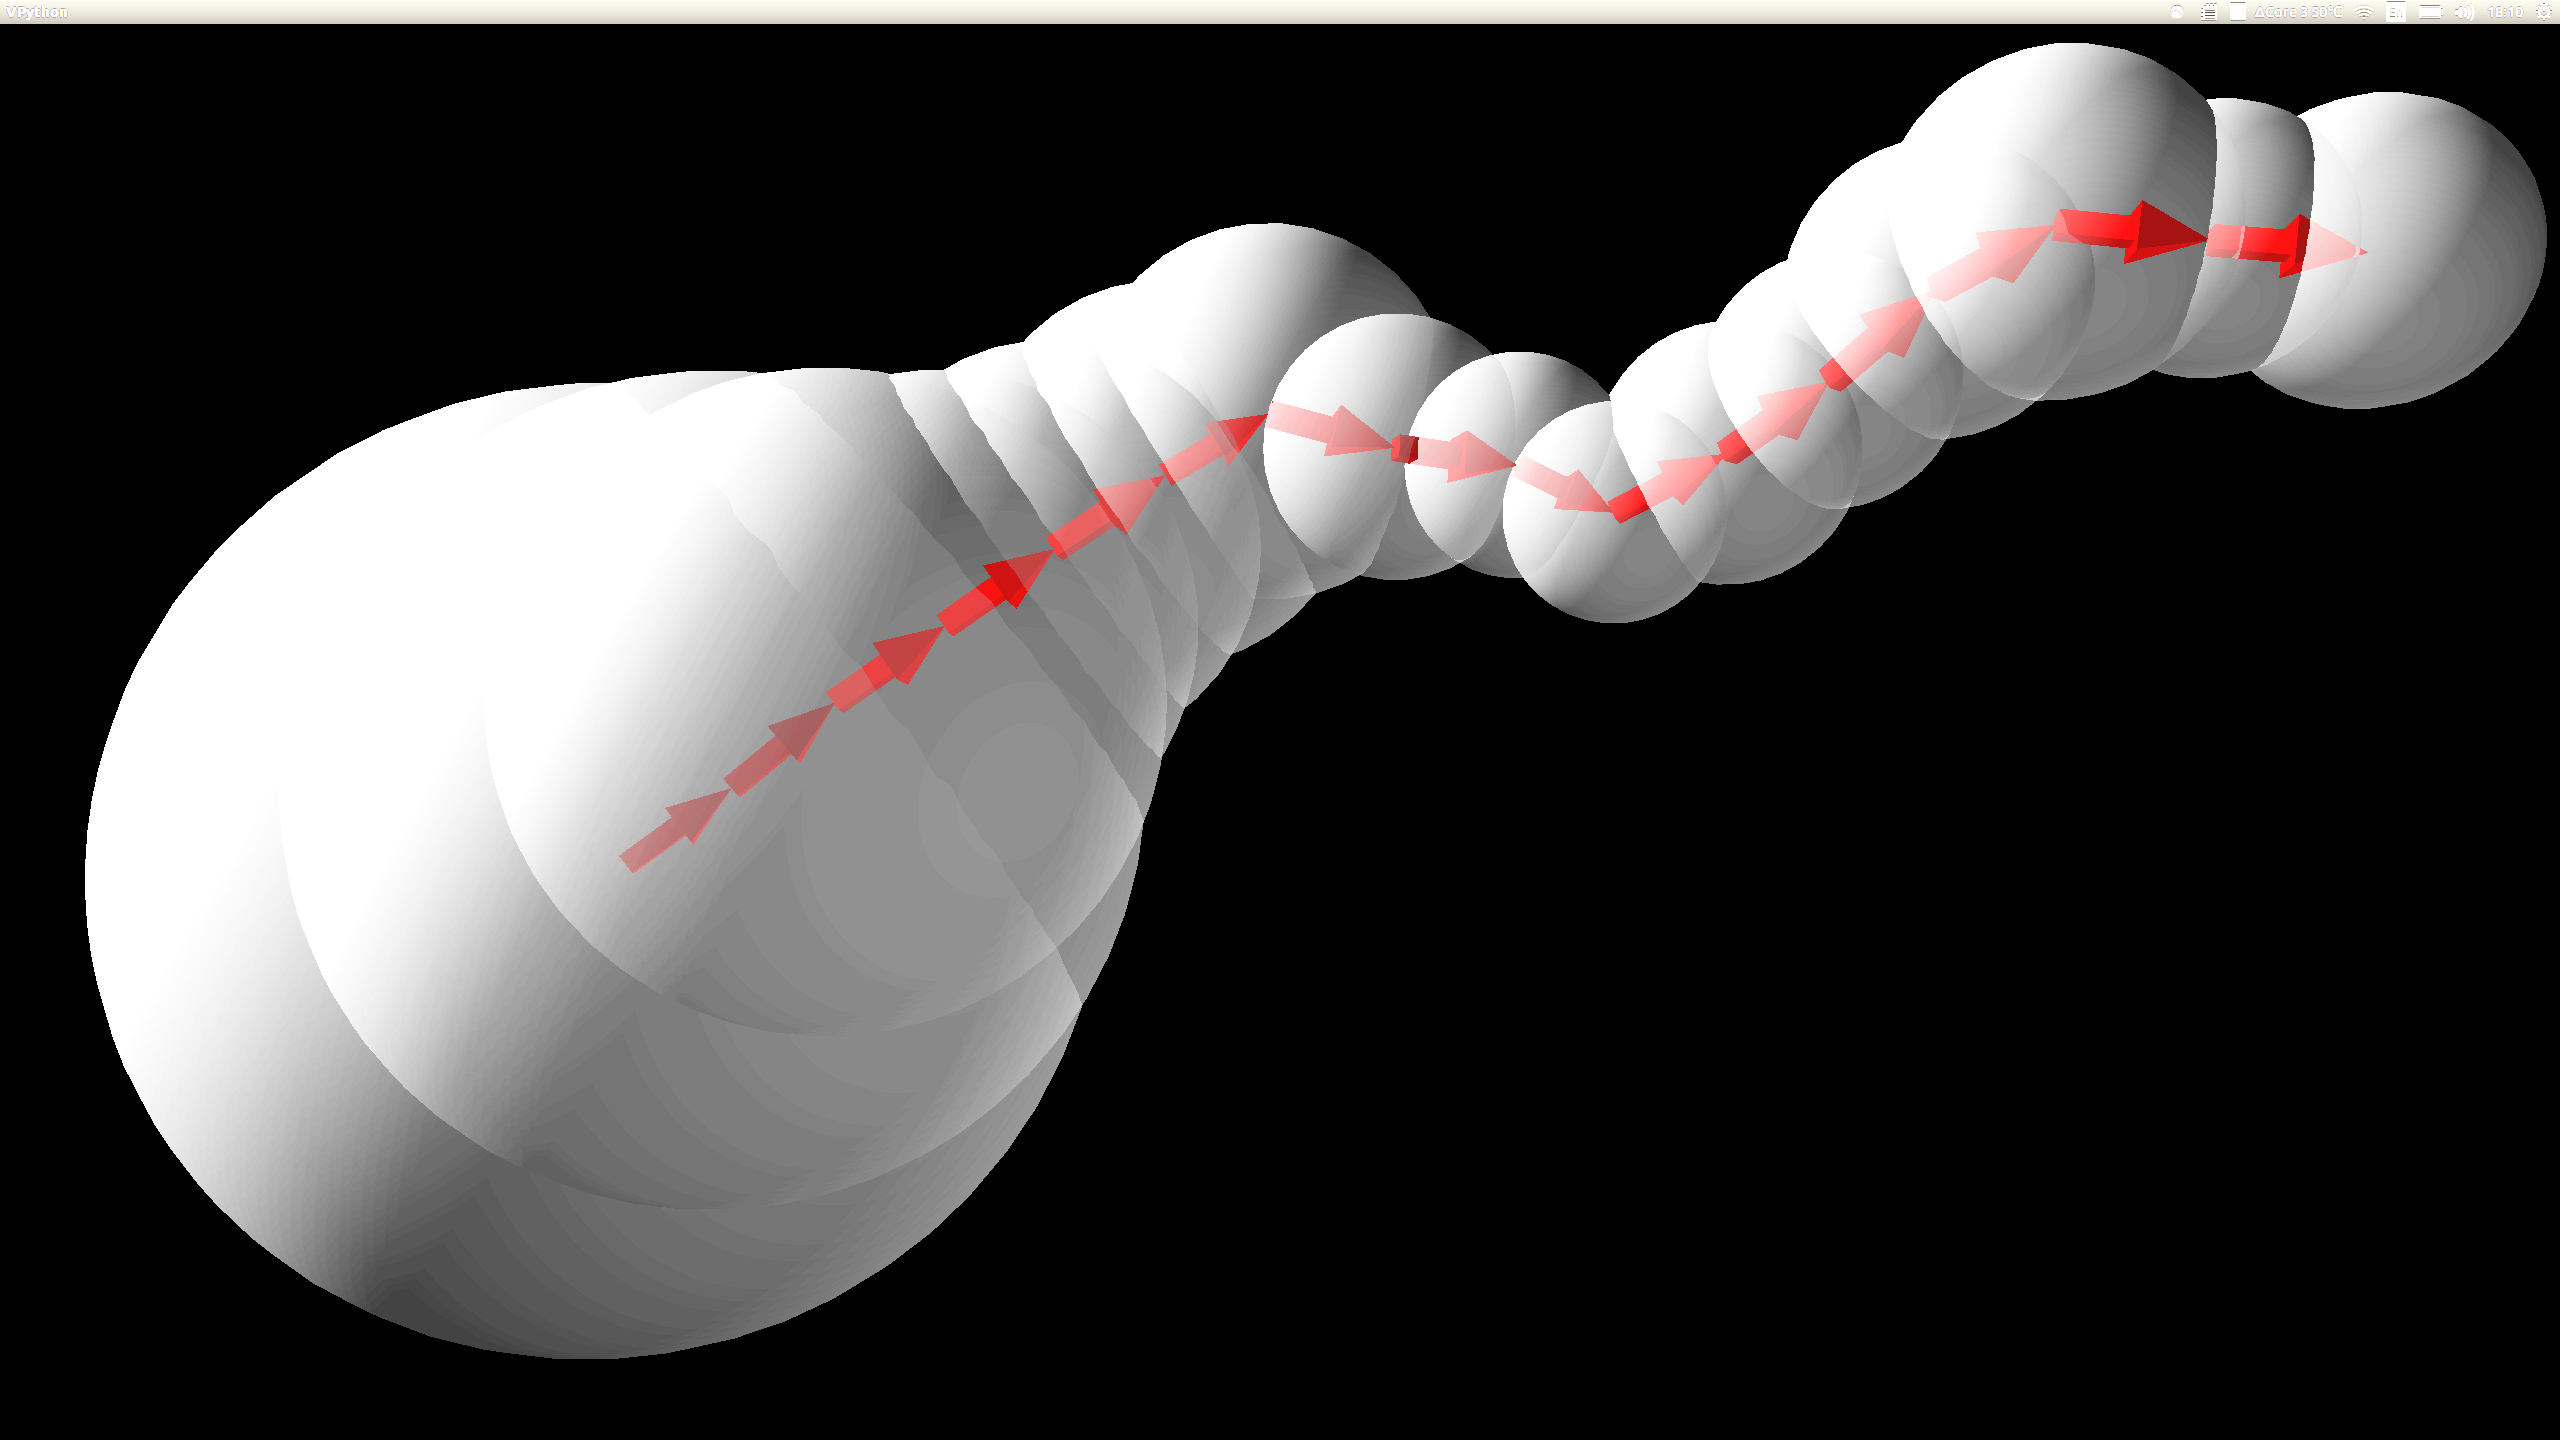
\includegraphics[width=100mm]{img/basic_tunnel.jpg}
	\caption{Sample of molecule tunnel}
  \centering
  \label{fig:basic_tunnel}
\end{figure}


Abychom mohli provádět docking ligandu, musíme nejprve takto definovaný tunel nařezat na jemné plátky - kruhy, na které pak v průběhu výpočtu budeme dokovat průběžné konformace ligandu. Popišme si nyní, jak by takové řezy měly vypadat.

\begin{defi}
Řezem tunelu $ \Tau $ rozumíme kruh v prostoru, který je určen uspořádanou trojicí $\theta = (A, u, r)$, kde $ A $ je střed, $ u \in \Rbb^3 $ je normálnový vektor a $ r > 0 $ je poloměr.
Pro tento kruh $ \theta $ musí platit, že $ \Tau \cap \theta $ je souvislá množina a navíc
$ \exists \delta > 0 $ tak, že $ \forall \varepsilon > 0,  \varepsilon < \delta $ je  $ (A, u, r + \varepsilon) \cap \Tau = \theta \cap \Tau $.
(Alternativně řečeno $\Tau \setminus \theta $ má dvě komponenty.)
\end{defi}

Uvedená definice prakticky říká, že řez tunel řeže jen na jednom místě (podmínka souvislosti). Druhá podmínka znamená, že řez je úplný, tedy že řezem skutečně rozdělíme tunel na dvě části.
Pro ilustraci, jak takové řezy mohou vypadat, přikládáme obrázek č. \ref{fig:tunnel_cuts}.
\begin{figure}[ht]
    \centering
    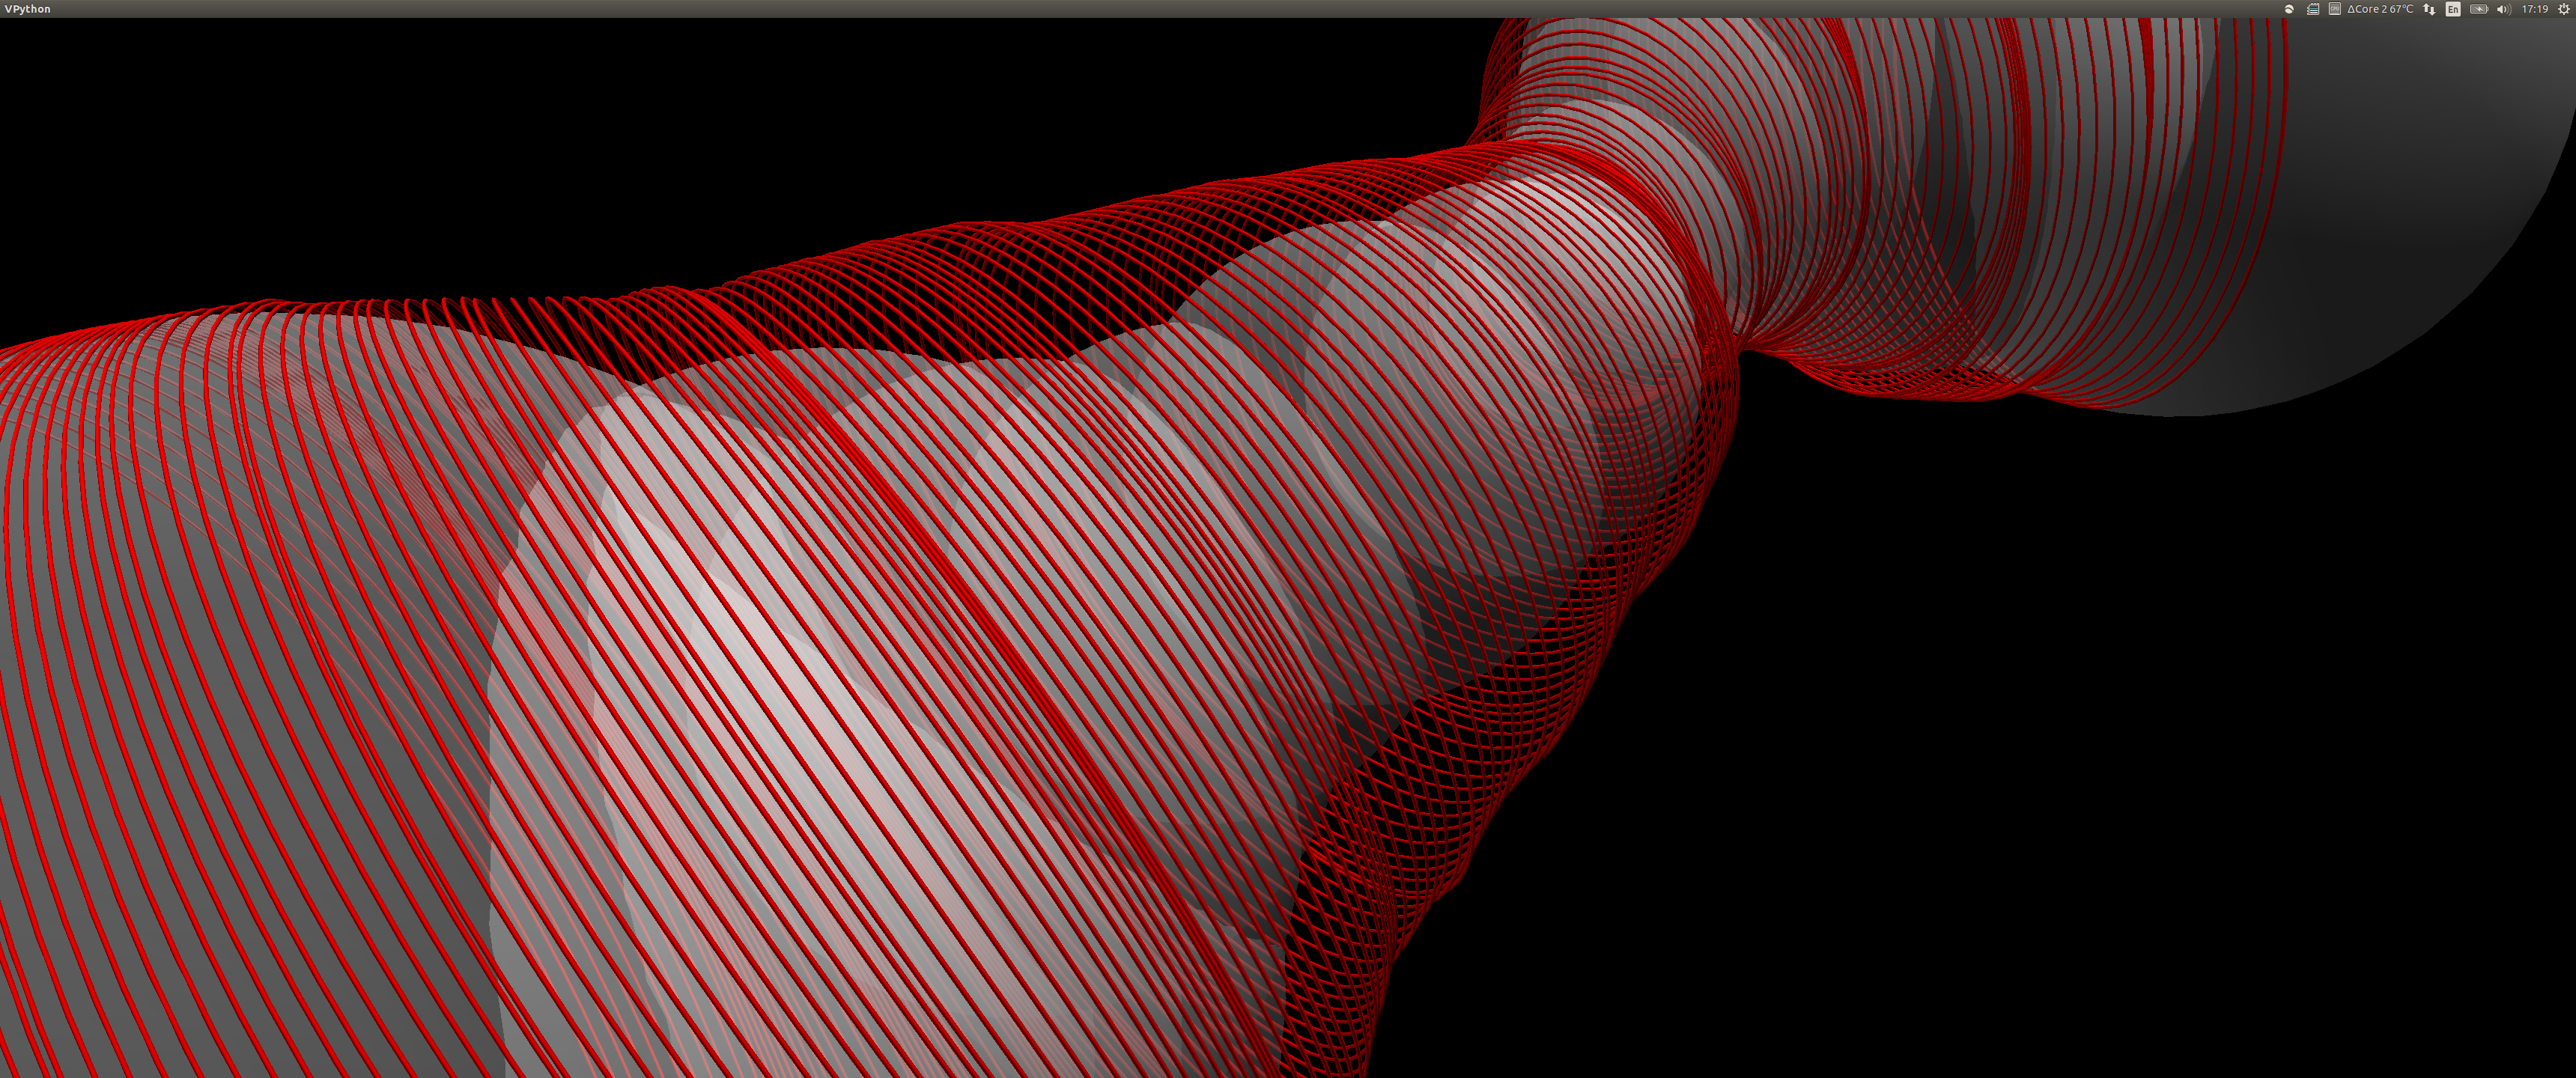
\includegraphics[width=\textwidth]{img/simple_cuts.png}
    \caption{Sample of molecule tunnel}
  \centering
  \label{fig:tunnel_cuts}
\end{figure}

S takto definovanými řezy můžeme začít uvažovat o tom, jak tunel nařezat jako celek.
Mějme $ \Theta = \{\theta_i\}_{i=0}^{k}$ posloupnost řezů tunelu $ \Tau $. Pro potřeby správného
dockingu bude nezbytné, aby platilo $ x, y \in \Theta \Rightarrow |x \cap y| \leq 1 $,
tedy každé dva řezy se dotýkají nejvýše v jednom bodě. Dále budeme chtít, aby po sobě
jdoucí řezy od sebe \textit{nebyly příliš daleko}. Vzdálenost budeme měřit pomocí funkce
$ \dst(x, y) $, kterou popisuje následující definice.

\begin{defi}
Mějme řezy $ x = (A, u, r_1), y = (B, v, r_2) \in \Theta $. Rozlišíme dvě situace
    \begin{enumerate}[label={(\arabic*)}]
        \item $ u = v $, pak vezmeme libovolný vektor $ w $ tak, aby
            $ \varrho = \langle u, w \rangle $ tvořilo rovinu.
        \item V opačném případě položíme přímo $ \varrho = \langle u, v \rangle $.
    \end{enumerate}
Kolmou projecí do roviny $ \varrho $ promítneme řezy $x $ resp. $y$, čímž získáme dvě úsečky
určené vrcholy $X_1, X_2 $ resp $Y_1, Y_2 $. Vzdálenost pak definujeme jako
    \begin{center}
        $ \dst(x, y) = \min\{ \max\{|X_1 - Y_1|, |X_2 - Y_2|\}, \max\{|X_1 - Y_2|, |X_2 - Y_1|\}\}$.
    \end{center}
\end{defi}

Nyní můžeme přistoupit k popisu samotného algoritmu, který má na vstupu tunel $ \Tau $
a nějaké pevně zadané $ \delta > 0$, které určuje maximální vzdálenost, kterou
od sebe dva po sobě jdoucí řezy mohou mít. Na výstupu pak budeme očkávat řezy pokrývající
celý tunel a budou splňovat uvedené omezení na vzdálenost. Vzhledem k tomu, že výsledná
složitost následného dockingu je přímo úměrná počtu řezů, budeme od algoritmu také chtít,
aby počet řezů byl při splnění uvedených kritérií pokud možno co nejmenší.


\subsection{Algoritmus}

Celý algoritmus se sestává z celé řady funkcí řešících méně či více důležité podproblémy.
Domníváme se, že vyčerpávající popis všech komponent by byl zbytečně technický a snad i
ubíjející, proto se zde zaměříme zejména na popis těch opravdu klíčových, zajímavých
a tam, kde implementace nějakého výpočtu nebude důležitá pro pochopení fungování
algoritmu jako celku, se omezíme pouze na symbolický zápis, případně stručný slovní
popis.

Pro začátek si řekněme něco o základní kostře algoritmu. Přirozeným naivním přístupem
k řešení našeho problému, by bylo vzít trajektorii tunelu tvořenou středy koulí
jím definované, po této trajektorii se s krokem $ \delta $ posouvat a generovat
řezy se středem na trajektorii a normálou určenou směrem pohybu na trajektorii.
Takovýto přístup by fungoval vcelku dobře pro tunely, které by byly relativně
přímé bez zatáček, avšak pro \say{klikaté} tunely by generoval řezy zcela nepoužitelné.
Pro ilustraci uvádíme obrázek \ref{fig:naive_cuts}.

\begin{figure}[ht]
    \centering
    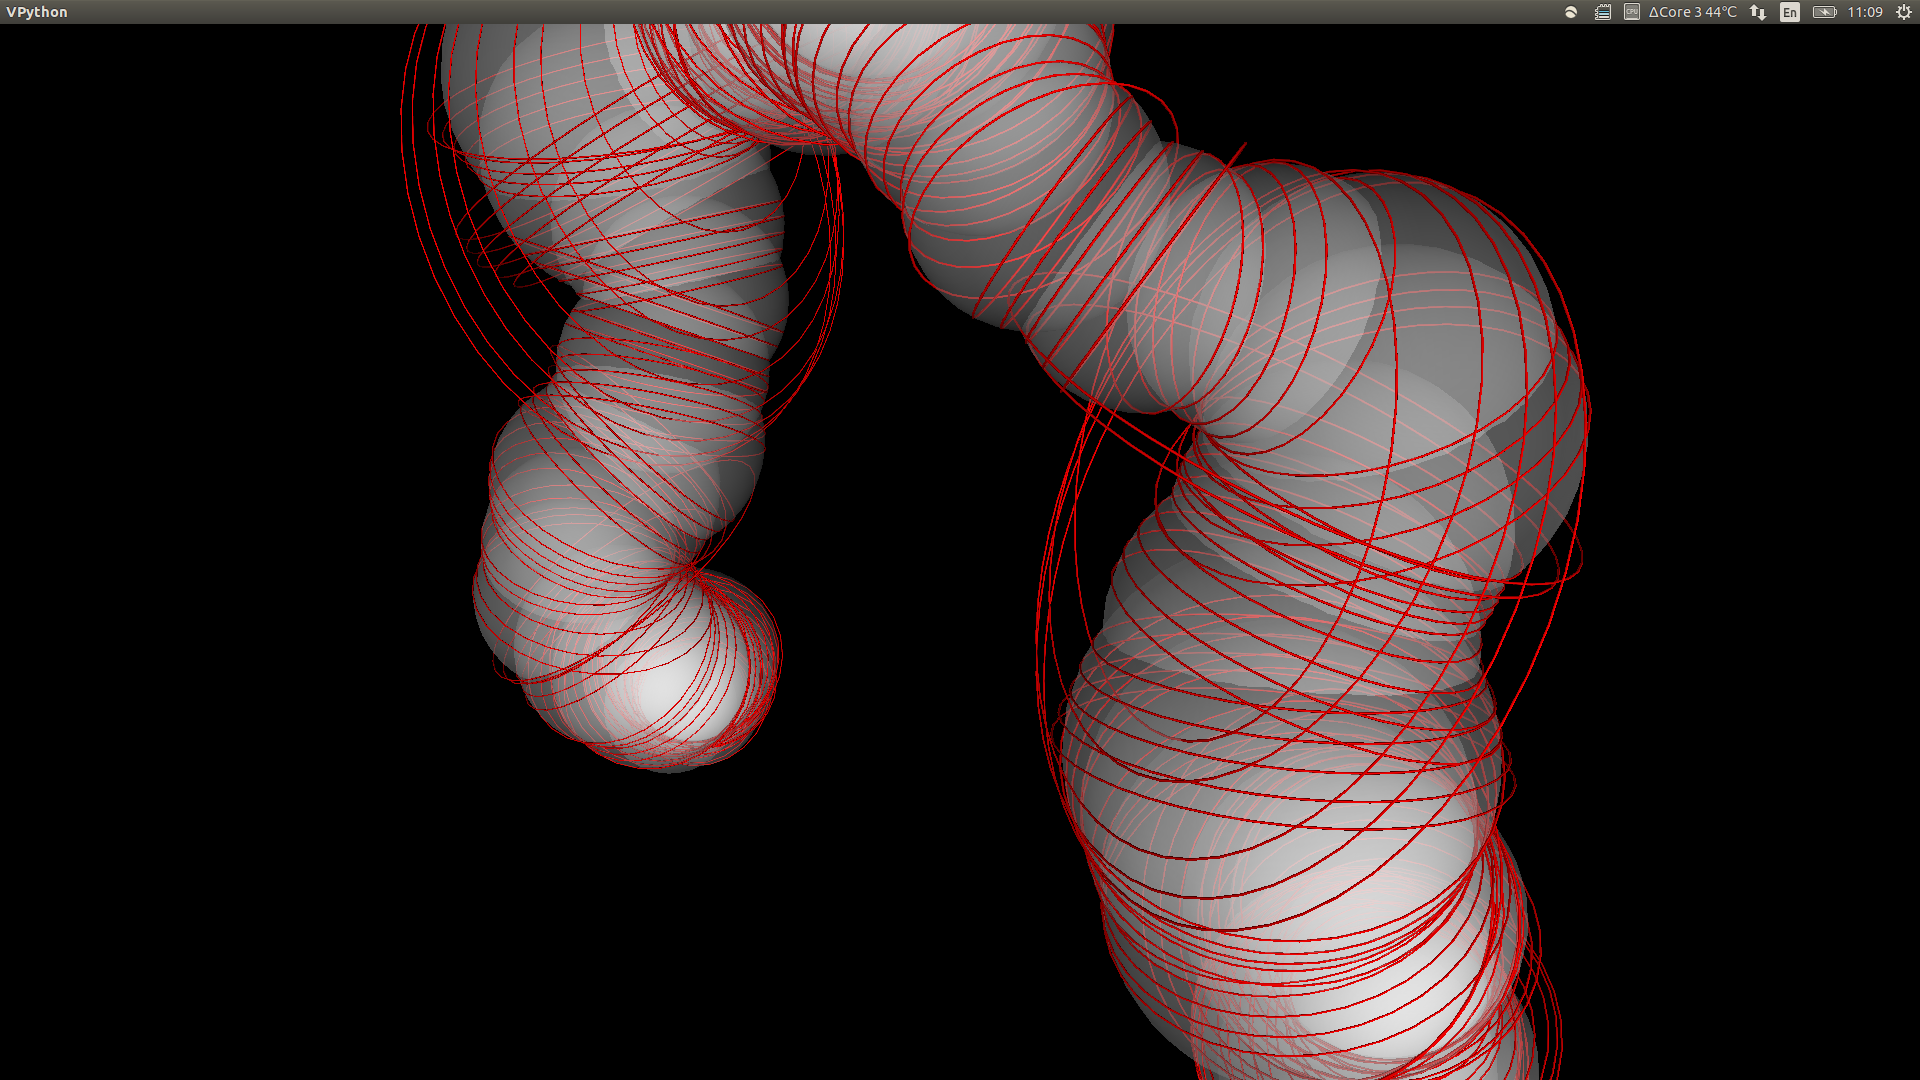
\includegraphics[width=\textwidth]{img/naive_cuts.png}
    \caption{Naive cuts}
  \centering
  \label{fig:naive_cuts}
\end{figure}

K problémům docházi proto, že bere v potaz pouze velmi lokální informace o vlastnostech
tunelu a zřejmě zcela ignorujeme dříve uvedené požadavky na řezy. Tento postup ale
můžeme zdokonalit. Prvním problémem je, že když takto postupně generujeme nové řezy,
může se stát, že od sebe budou příliš daleko nebo se budou protínat. Potřebujeme proto
funkci $ shiftNewDisk $, která přesně toto zajistí. Jak ale můžeme vidět na obrázku
\ref{fig:shift_cuts}, toto způsobí, že se v případě nevhodné orientace normálových
vektorů sice zachovají naše požadavky na řezy, avšak dostaneme jich zbytečně mnoho.

\begin{figure}[ht]
    \centering
    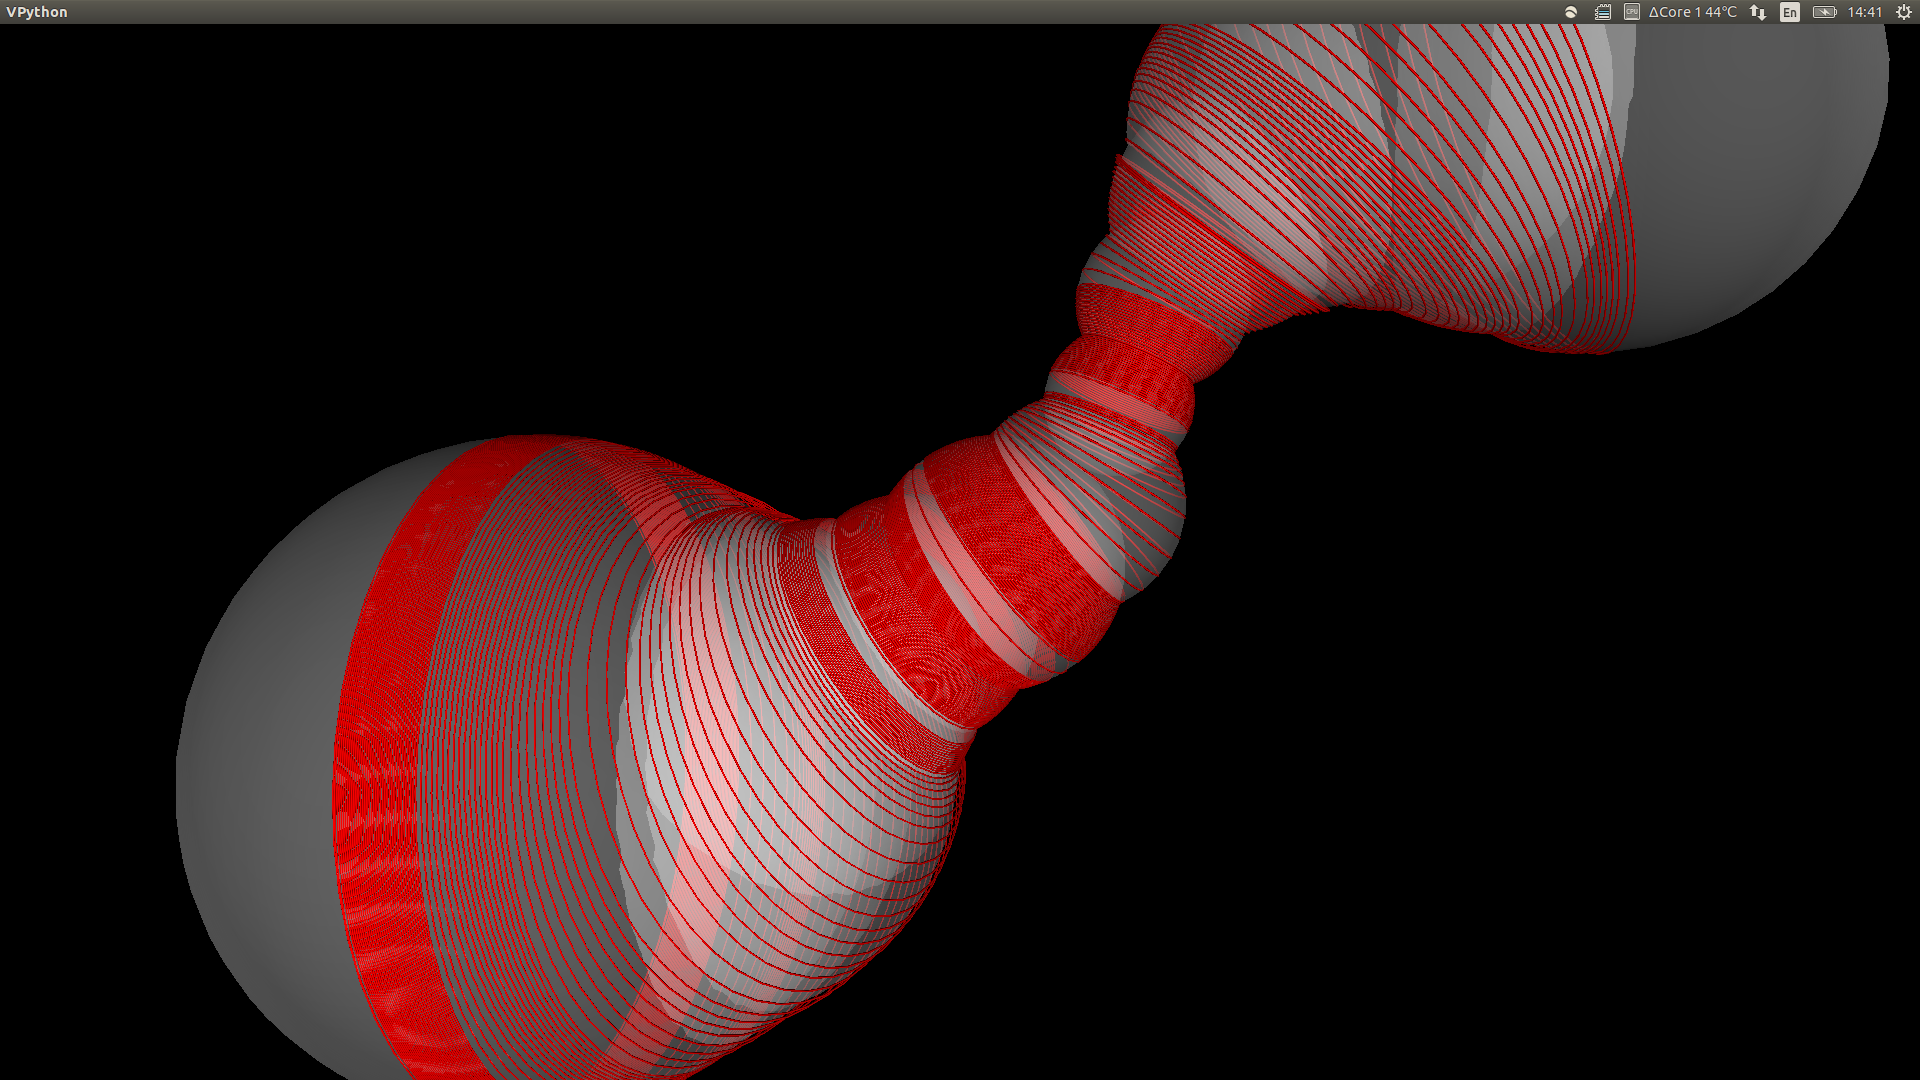
\includegraphics[width=\textwidth]{img/shift_cuts.png}
    \caption{Shifting cuts}
  \centering
  \label{fig:shift_cuts}
\end{figure}

Z toho důvodu je ještě vhodné po každém posunu zkontrolovat, zda nemůžeme předchozí
řez prostě jen nahradit novým řezem $ \theta $. To jest pro
$ \theta_{i - 2} \in \Theta $ zkontrolovat zda náhodou neplatí
$ \dst(\theta_{i - 2}, \theta) < \delta $. Pokud ano, můžeme zřejmě nahradit
$ \theta_{i - 1} = \theta $. (Toto má samozřejmě smysl jen pokud
$ |\Theta| > 1 $.) Jak můžeme vidět na obrázku \ref{fig:cuts_with_replace}
výsledek již vypadá o mnoho lépe.

\begin{figure}[ht]
    \centering
    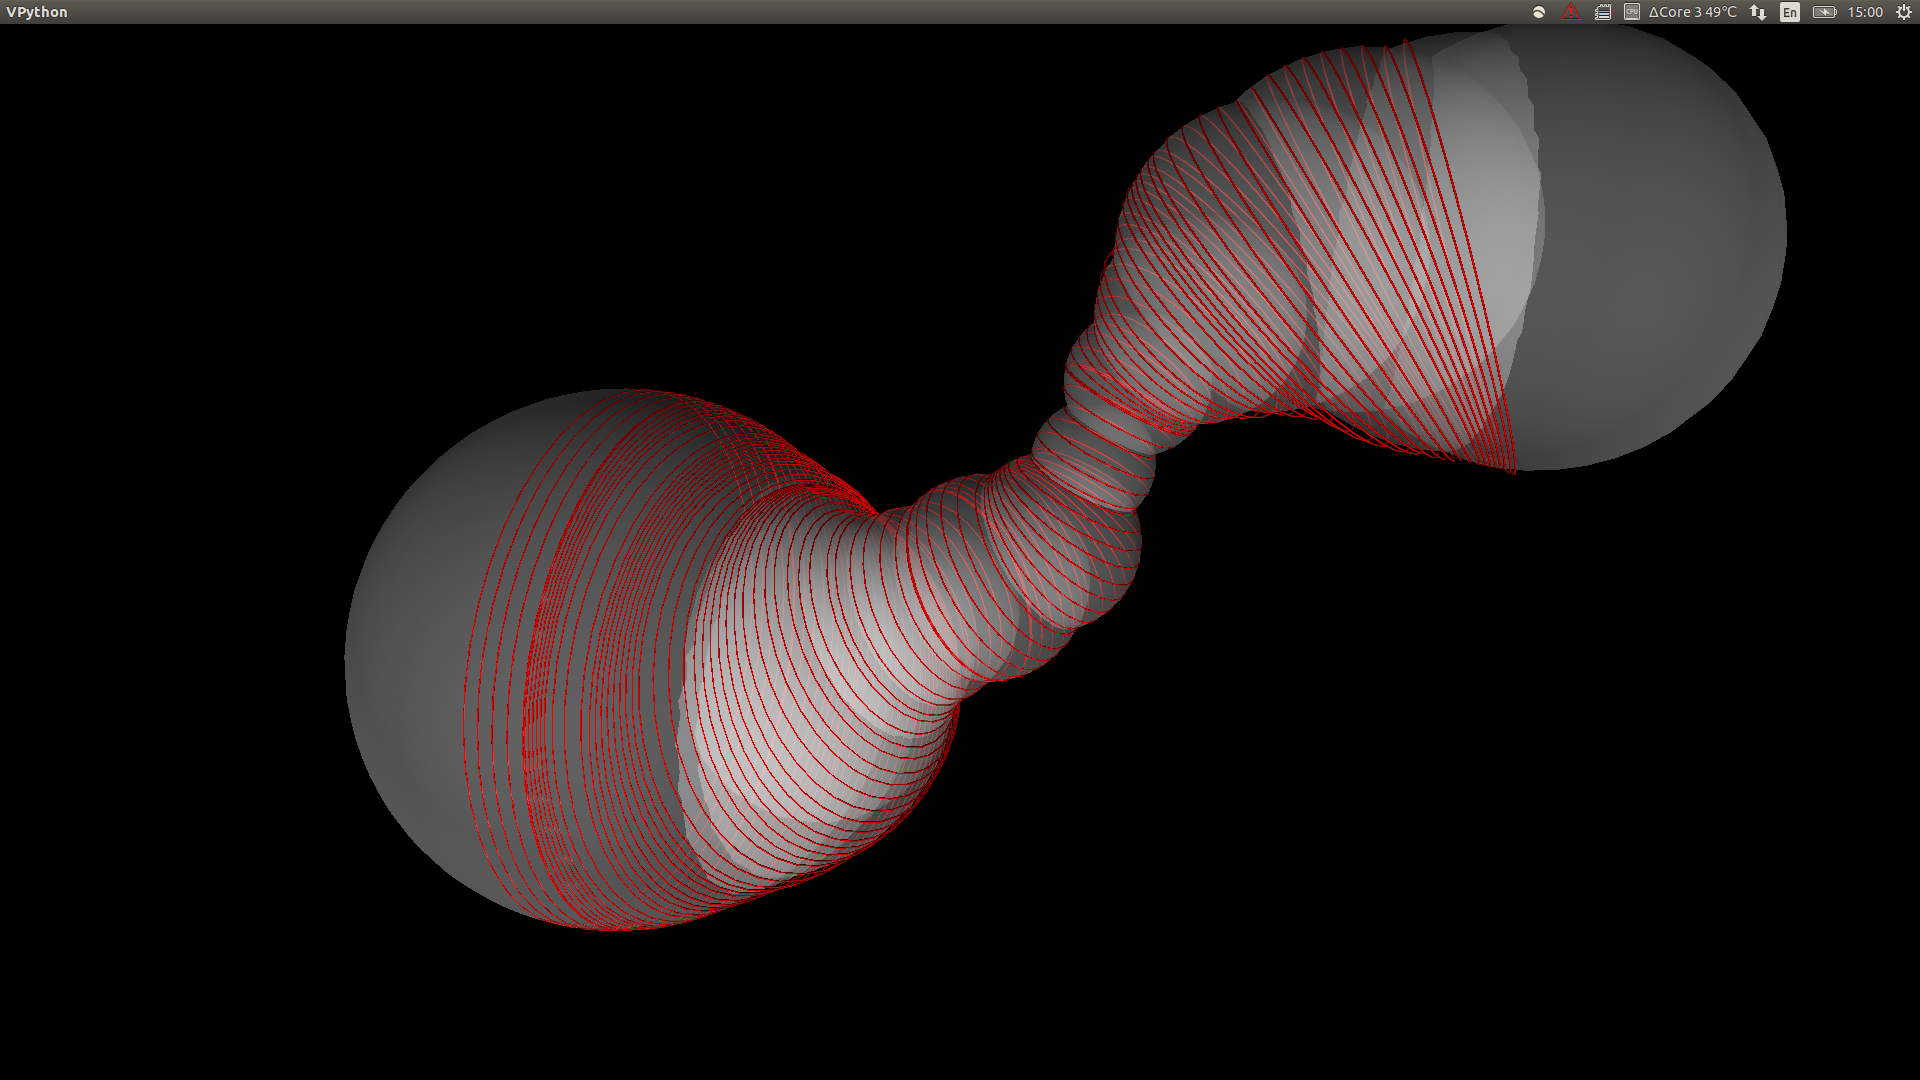
\includegraphics[width=\textwidth]{img/cuts_with_replace.png}
    \caption{Cuts with replace}
  \centering
  \label{fig:cuts_with_replace}
\end{figure}

Jak si ale pozorný čtenář může povšimnout, na pravém konci tunelu uvedeného na
posledním obrázku můžeme vidět, že řezy nezatáčí tak jak by mohly a nekopírují tak
profil tunelu příliš věrně. Po krátkém zamyšlení se dá nahlédnout, že tomu tak
je pravděpodobně kvůli tomu, jaké volíme výchozí normálové vektory pro jednotlivé
řezy. Pokud řezy orientujeme výhradně podle lokálních vlastností trajektorie,
tak se nám může stát, že právě například nezačneme zatáčet dostatečně brzy apod.
Z tohoto důvodu budeme pro výpočet normály nového řezu používat třídu
$ TunnelCurve $ a její metodu $ getWeightedDir $, která pro daný bod $ P $ na křivce
- trajektorii tunelu spočítá vážený průměr směrových vektorů této křivky na
okolí bodu $ P $. Exaktněji tento výpočet a případná zlepšení rozvedeme později.
Pro ilustraci se ještě podívejme na obrázek \ref{fig:weighted_dir}. Je vidět, že
řezy nyní kopírují zakřivení tunelu mnohem ochotněji.

\begin{figure}[ht]
    \centering
    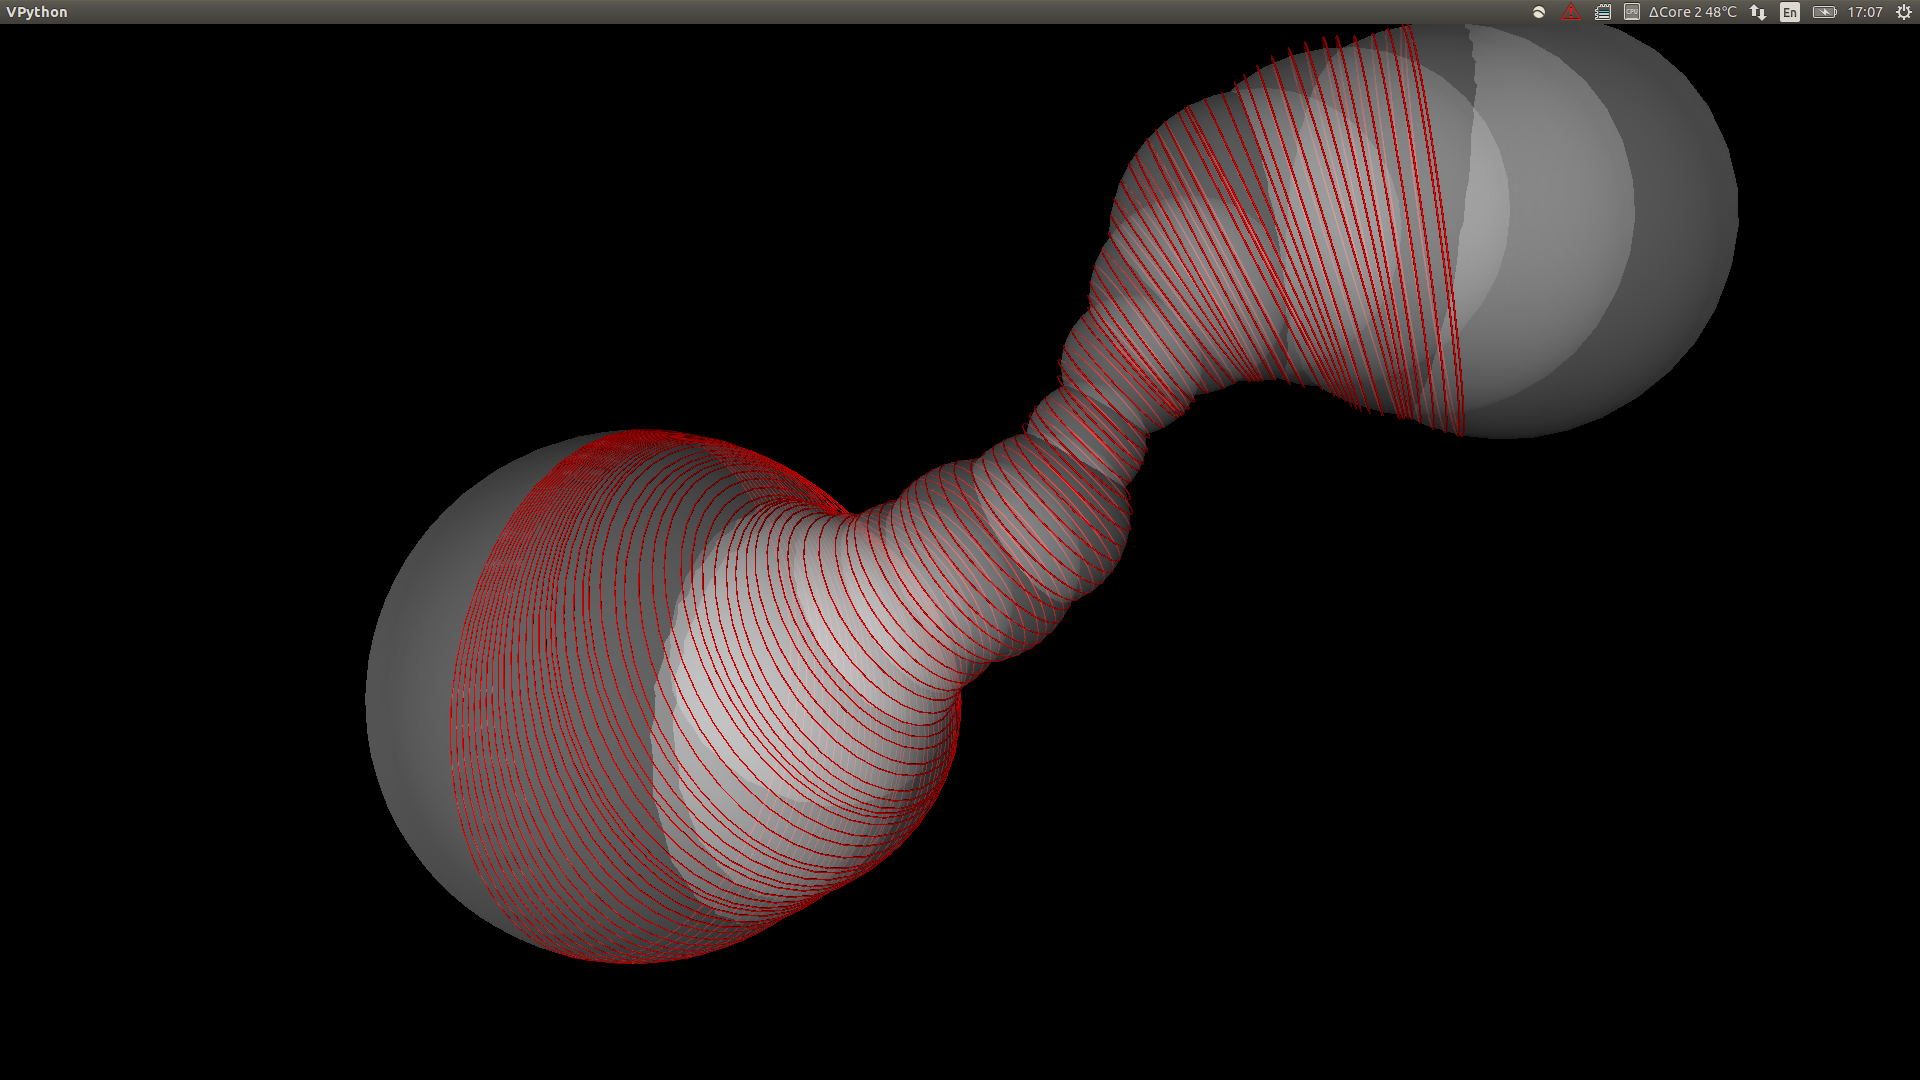
\includegraphics[width=\textwidth]{img/weighted_dir.png}
    \caption{Cuts with weighted direction}
  \centering
  \label{fig:weighted_dir}
\end{figure}

Kostru naznačeného algoritmu zachycuje následující pseudokód.

\begin{algorithmic}[1]
\label{alg:digTunnel}

\Function{digTunnel}{$\Tau, \delta$}
    \State $ centers \gets [ S_{center} \in \Tau ] $
    \State $ normals \gets [ \operatorname{norm}(C_{i + 1} - C_{i}) \mid 0 \leq i < |centers| ] $
    \State $ disks \gets   [ \operatorname{fitDiskTunnel}(normals[0], centers[0], \Tau, \delta)] $
    \State $ curve \gets \operatorname{TunnelCurve}(centers) $
    \Statex

    \For{$ S_i \in \Tau $}
        \If{$ i = |T| - 2 $}
            \Break
        \EndIf
        \State $ \vec{n} \gets normals[i] $
        \State $ center \gets centers[i] $
        \State $ dir \gets centers[i + 1] - center $
        \State $ line \gets \operatorname{Line}(center, dir) $
        \Statex

        \State $ size \gets 0 $
        \While {$ size < \norm{dir} $}
            \If{$ size \neq 0 $}
                \State $ plane \gets \operatorname{getPlane}(disks[-1]) $
                \State $ size \gets \dis(plane \cap line, center) + \epsilon $
            \EndIf
            \Statex

            \State $ disk\_center \gets center + normal * size $
            \State $ disk\_normal \gets \operatorname{getWeightedDir}(curve, i, size) $

            \State $ disk \gets \operatorname{fitDiskTunnel}(disk\_normal, disk\_center) $ \label{alg:fit_disk}
            \State $ disk \gets \operatorname{shiftDisk}(disk, disks[-1]) $
            \Statex

            \If{$ |disks| > 1  \And \dst(disk, disks[-2]) < \delta $}
                \State $ disks[-1] \gets disk $
            \Else
                \State $ \operatorname{Push}(disks, disk) $
            \EndIf
            \State $ size \gets size + \epsilon $
        \EndWhile
    \EndFor
    \State \Return $ disks $
\EndFunction

\end{algorithmic}

Výsledný algoritmus tedy iterativně prochází tajektorii tunelu a postupně vytváří řezy
se středem iniciálně umístěným na trajektorii, které pak v případě potřeby posune tak,
aby byly zachovány námi požadované podmínky.

Dříve než budeme pokračovat v dalším popisu, rozvedeme dva dříve neokomentované
detaily kostry algoritmu. První věcí, které si čtenář mohl povšimnout, je použití přímky
$ line $. Díky výpočtu průsečíku roviny určené předchozím řezem s touto přímkou, se
vždy posuneme tunelem vpřed, a to před předchozí řez. Druhým detailem je použití
konstanty $ \epsilon $. Ta udává s jakým krokem se budeme tunelem pohybovat.
Volíme ji tak, aby platilo  $ \epsilon < \delta $, byla dostatečně malá abychom
předešli zaokrouhlovacím chybám, ale zároveň čím větší bude, tím rychleji se
budeme tunelem pohybovat a tím rychleji také celý algoritmus doběhne. Experimentálně
jsme ověřili, že vhodnou volbou je například $ \epsilon = \frac{9}{10} \delta $.


\subsection{Disk fitting}
Nyní se budeme věnovat funkci $ \operatorname{fitDiskTunnel} $ použité na řádku
\ref{alg:fit_disk}. Na tomto místě již víme jaký normálový vektor by měl řez mít a
zároveň máme k dispozici referenční bod $ P $, který nám společně s normálou
určuje rovinu $ \rho $. Našim úkolem je najít střed a poloměr řezu tak, aby
byly splněny požadované podmínky a zároveň aby byl poloměr řezu co nejmenší.

První věc, kterou musíme vyřešit je, že rovina $ \rho $ může protínat tunel $ \Tau $
na více místech, avšak nás zajímá jen okolí bodu $ P $. Do tohoto okolí jistě
budou patřit ty koule, které bod $ P $ přímo obsahují. Explicitně
zapsáno $ C = \{S_i \in \Tau \mid P \in S_i \} $. Dále musíme pokrýt všechny
koule které mají neprázdný průnik s rovinou $ \rho $ a některou z koulí z $ C $.
Celkem dostáváme
$ O = \{ S_i \in \Tau \mid S_i \cap \rho \neq \emptyset \wedge \exists S \in C \colon S \cap S_i \neq \emptyset  \}$
Tímto způsobem pokrýváme rozumné okolí bodu $ P $. To sice v případě špatného
natočení normálového vektoru a extrémně zakrouceného tunelu nemusí stačit, ale
experimenty ukazují, že tento přístup je naprosto dostatečný a v praxi funguje
naprosto spolehlivě.

Teď když víme, které koule jsou pro nás relevantní, uvážíme průřez rovinou
$ \rho $ koulemi z $ O $. Každá z těchto koulí v uvažovaném řezu vykreslí
kružnici (nebo jediný bod, který ale můžeme považovat za speciální případ kružnice).
Náš problém se tak redukuje na planární úlohu konstrukce minimální kružnice obsahující
všechny zadané kružnice. Jak se v práci Kaspara Fishera \cite{FisherBalls} ukazuje,
jedná se o silně netriviální problém. Zde si nastíníme dvě možnosti jeho řešení.

Jednodušší přístup spočívá v aproximaci kružnic pomocí dostatečného množství bodů
rovnoměrně rozložených po jejich obvodu. Můžeme například požadovat, aby dva
po sobě jdoucí body od sebe nebyly vzdáleny o více než $ \frac{\delta}{10} $.
Pro tyto body pak můžeme použít například Welzlův náhodnostní algoritmus
\cite{WelzlRandom}, jehož očekávaná doba běhu je v $ \mathcal{O}(n) $. Tento
přístup byl první, který jsme zkusili, protože implementace níže uvedeného algoritmu
existuje (alespoň pokud je nám známo) pouze v C++ a naším výchozím jazykem byl
Python. O tomto budeme ještě hovořit později.

Složitější, ale přesnější způsob popisuje již zmíněná práce Kaspara Fishera
\cite{FisherBalls}. Zde je problém řešen v plné obecnosti libovolné dimenze $ d $.
Popsaný algoritmus dosahuje očekávané doby běhu
$ \mathcal{O}(d^2n) + e^{\mathcal{O}(\sqrt{d \log{d}})} $. V našem případě tak pro
$ d = 2 $ dostáváme velmi efektivní algoritmus. K dispozici je dokonce velice
robustní C++ implementace dostupná z \cite{cpp_balls}, která podle uvedených informací
zvládá řešit úlohy ve 3D o velikosti 1 milionu koulí v čase pod 1 sekundu. To
je rozhodně velmi působivý výsledek.

Výše uvedené pak můžeme vyjádřit pomocí jednoduchého pseudokódu \ref{alg:fitDiskTunnel}.

\begin{algorithmic}[1]
\label{alg:fitDiskTunnel}

\Function{fitDiskTunnel}{$ \vec{n}, P$}
    \State $ \rho \gets Plane(\vec{n}, P) $
    \State $ C \gets \{S_i \in \Tau \mid P \in S_i \} $
    \State $ O \gets \{ S_i \in \Tau
        \mid S_i \cap \rho \neq \emptyset
            \wedge \exists S \in C \colon S \cap S_i \neq \emptyset  \} $
    \State $ circles \gets \{ \operatorname{Circle}_{\rho}(S \cap \rho) \mid S \in O \} $
    \State

    \State $ Q, radius \gets \operatorname{getMinCircle}(circles) $
    \State \Return $ \operatorname{Disk}(\vec{n}, \rho(Q), radius) $
\EndFunction

\end{algorithmic}

Poznamenejme, že $ \operatorname{Circle}_{\rho} $ značí konstrukci 2D kružnice
v parametrizaci roviny $ \rho $, $ \operatorname{getMinCircle} $ je některý z
uvedených algoritmů pro nalezení minimální kružnice (vrací střed a poloměr)
a konečně $ \rho(Q) $ značí převod bodu $ Q $ (středu) z lokálních souřadnic
roviny $ \rho $ do souřadného systému původního prostoru.

